\subsection{Required precision} \label{sec:RequiredPrecision}
As of \autoref{ch:ProblemStatement} a laser pointer is made available for this project. It is chosen that the goal is to hit the drone with it. 

In this subsection the required precision to hit the drone with the laser pointer is determined. This requirement is the criterion to evaluate the feasibility of the different tracking methods in the later part of this chapter. 
 
The trigonometric model on \autoref{fig:RequiredPrecision} is made to calculate the required precision when the beam is pointing at the center of the drone. 
\begin{figure}[h!]
    \centering
        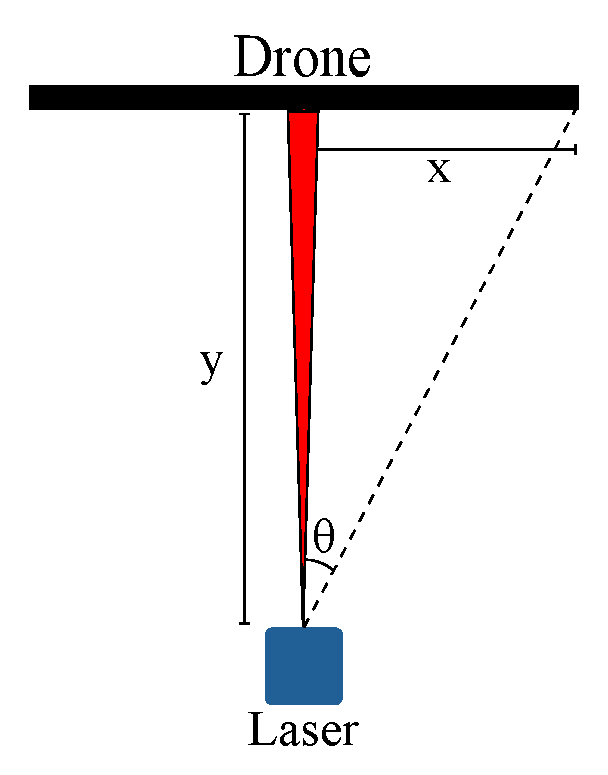
\includegraphics[width=0.4\textwidth]{figures/tracking/required_precision.pdf}
        \caption{Illustration of the laser pointing at the drone. $\theta$ is the maximum angular deviation the tracking module can have while still hitting the target.}
        \label{fig:RequiredPrecision}
\end{figure}

\newpage
From \autoref{fig:RequiredPrecision} \autoref{eq:GeneralRequiredPrecision} is derived. 
\begin{equation} \label{eq:GeneralRequiredPrecision}
\theta = \arctan \left( \frac{x}{y} \right) \addunit{\radian}
\end{equation}
\startexplain
\explain{$\theta$ is the angular precision}{\si{\radian}}
\explain{$x$ is half the size of the drone}{\si{\meter}}
\explain{$y$ is the distance from the laser to the drone}{\si{\meter}}
\stopexplain
Because the laser is purely for demonstration purposes, beam spreading is not taken into account. 

In order to calculate the required precision a choice of the maximum operation range of the drone is needed. Since the system is a charging station for a drone it is assumed that the drone is able to move to the charging station. Since this is a proof of concept, it is chosen that a maximum operation range of \SI{120}{\meter} is sufficient. \SI{120}{\meter} is chosen because it is approximately the maximum altitude of the 3DR Solo drone. 

With the maximum operation distance of \SI{120}{\meter} and a drone size of approximately \SI{500}{\milli\meter}, \autoref{eq:GeneralRequiredPrecision} can be used to calculate the required precision, as seen in \autoref{eq:RequiredPrecision}. 
\begin{equation}\label{eq:RequiredPrecision}
\theta_{\SI{120}{\meter}} = \arctan \left( \frac{{\dfrac{\SI{500}{\milli\meter}}{2}}}{\SI{120}{\meter}} \right) \approxeq \SI{2,083}{\milli\radian} 
\end{equation}
 

Now the required precision is found to be \SI{2.083}{\milli\radian} and the needed angular velocity is researched.